\subsection{Gerichteter Multigraph}
\subsubsection{Motivaton}
Graphen sind ein gutes Modell für verschiedene Problemstellungen.
Wie jedes Modell dienen sie dazu, die Realität zu simplifizieren und auf das Wesentliche zu beschränken.
Bei einem Netzwerk wäre eine geeignete Abstraktion, dass man sich auf die Betrachtung von Objekten(die als Knoten bezeichnet werden) und ihrer Verbindungen beschränkt.
Die Position der Knoten ist nicht relevant.


\subsubsection{Definition}
Ein \emph{gerichteter Multigraph}(auch: Netzwerk) $G:= (V,E,\sigma,\tau) $ besteht aus einer \emph{Knotenmenge} $V$, einer \emph{Kantenmenge} $E$ sowie
$\sigma , \tau , \in V^E $.
\\ $\sigma $ wird als source map(Anfangspunkt) von G bezeichnet.
\\ $\tau $ wird als target map(Endpunkt) von G bezeichnet.
\\ $\rho : E \rightarrow V \times V, e \mapsto (\sigma e, \tau e) $
\\
\\G heiße einfach, falls g injektiv ist.

\subsubsection{Erläuterungen zur Definition}
Im Gegensatz zu ungerichteten Graphen, werden bei der graphischen Darstellung eines Graphen Kanten durch Pfeile(und nicht durch Linien) dargestellt.
Dadurch soll verdeutlicht werden, dass man die Kante nur in eine Richtung(nämlich die Pfeilrichtung) ``durchlaufen'' kann.

Bei einem Multigraphen ist es - im Gegensatz zu einem einfachem Graphen - erlaubt, zwei Knoten auch durch mehrere Kanten zu verbinden.
Auch sogenannte Schlingen(eine Kante von einem Knoten auch sich selbst) sind erlaubt.

\subsubsection{Beispiel}
\subsubsection*{a)}
\begin{figure}[H]
  \begin{center}
  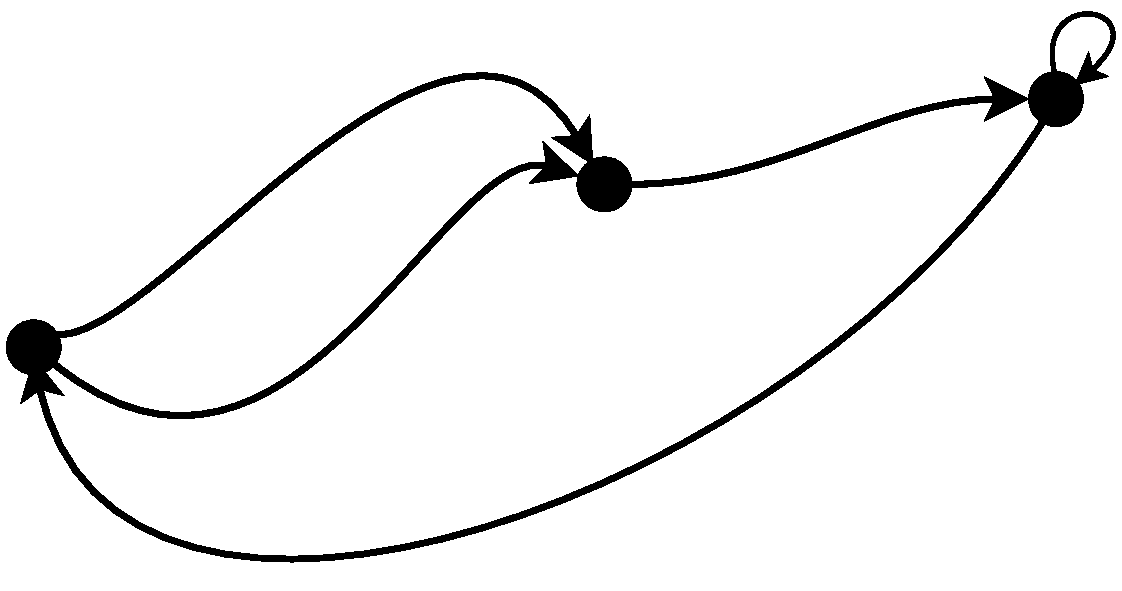
\includegraphics[scale=0.5,keepaspectratio=true]{../bilder/multigraph_bsp.pdf}
  % multigraph_bsp.pdf: 539x283 pixel, 72dpi, 19.01x9.98 cm, bb=0 0 539 283
 \end{center}
 \caption{Ein Beispiel für einen gerichteten Multigraphen: es sind sowohl Schlingen als auch mehrfache Verbindungen von zwei Knoten erlaubt}
\end{figure}

\paragraph{b)}
Sei V Menge und $E \subseteq V \times V $ ``binäre Relation auf V''
\\Dann ist $G(V,E) := (V,E, \sigma, \tau) $
\\mit $\sigma : E \rightarrow V, (p,q) \mapsto p$
\\und $\tau : E \rightarrow V, q \mapsto (p,q)$


